\documentclass[12pt, a4paper]{book}

\usepackage[T1]{fontenc}
\usepackage[utf8]{inputenc}
\usepackage[charter, cal=cmcal]{mathdesign}
\usepackage[scaled=0.92]{helvet}
\usepackage{geometry}
\geometry{a4paper, top=30mm, bottom=30mm, inner=32mm, outer=25mm, marginparwidth=18mm}

\usepackage{amsmath, amsthm}
\usepackage[version=4]{mhchem}
\usepackage{graphicx}
\usepackage[dvipsnames,svgnames,table]{xcolor}
\usepackage{tikz}
\usetikzlibrary{arrows.meta, shapes.geometric, positioning,
                calc, backgrounds, decorations.pathmorphing, patterns}
\usepackage{pgfplots}
\pgfplotsset{compat=1.18}
\usepackage{tcolorbox}
\tcbuselibrary{skins, breakable, theorems}
\usepackage{titlesec}
\usepackage{fancyhdr}
\usepackage{enumitem}
\usepackage{booktabs}
\usepackage{array}
\usepackage{multicol}
\usepackage{caption}
\usepackage{parskip}
\usepackage{siunitx}
\usepackage{pifont}
\usepackage[colorlinks=true, linkcolor=BrickRed,
            urlcolor=NavyBlue, citecolor=ForestGreen]{hyperref}

% ── Colours ───────────────────────────────────────────────────────────────────
\definecolor{JourneyColor}{HTML}{4A235A}
\definecolor{ModuleColor}{HTML}{6C3483}
\definecolor{PuzzleColor}{HTML}{1A5276}
\definecolor{DiscoveryColor}{HTML}{B7950B}
\definecolor{WarningColor}{HTML}{C0392B}
\definecolor{ProblemColor}{HTML}{117A65}
\definecolor{ReflectColor}{HTML}{1D6A39}
\definecolor{HistoryColor}{HTML}{6E2F1A}
\definecolor{LightBg}{HTML}{F8F9FA}
\definecolor{ElectronBlue}{HTML}{1565C0}
\definecolor{NucleusRed}{HTML}{B71C1C}
\definecolor{BohrOrbit}{HTML}{1A237E}

% ── Boxes ─────────────────────────────────────────────────────────────────────
\newtcolorbox{puzzlebox}[1][]{enhanced,breakable,
  colback=PuzzleColor!6,colframe=PuzzleColor,fonttitle=\bfseries\sffamily,
  title={The Puzzle},attach boxed title to top left={yshift=-2mm,xshift=6mm},
  boxed title style={colback=PuzzleColor},borderline west={3pt}{0pt}{PuzzleColor},#1}

\newtcolorbox{discoverybox}[1][]{enhanced,breakable,
  colback=DiscoveryColor!8,colframe=DiscoveryColor,fonttitle=\bfseries\sffamily,
  title={Discovery},attach boxed title to top left={yshift=-2mm,xshift=6mm},
  boxed title style={colback=DiscoveryColor},borderline west={3pt}{0pt}{DiscoveryColor},#1}

\newtcolorbox{problembox}[1][]{enhanced,breakable,
  colback=ProblemColor!5,colframe=ProblemColor,fonttitle=\bfseries\sffamily,
  title={Problems},attach boxed title to top left={yshift=-2mm,xshift=6mm},
  boxed title style={colback=ProblemColor},borderline west={3pt}{0pt}{ProblemColor},#1}

\newtcolorbox{deepbox}[1][]{enhanced,breakable,
  colback=JourneyColor!5,colframe=JourneyColor,fonttitle=\bfseries\sffamily,
  title={Deep Problems},attach boxed title to top left={yshift=-2mm,xshift=6mm},
  boxed title style={colback=JourneyColor},borderline west={4pt}{0pt}{JourneyColor},#1}

\newtcolorbox{historybox}[1][]{enhanced,breakable,
  colback=HistoryColor!7,colframe=HistoryColor!60,fonttitle=\bfseries\sffamily\small,
  title={Historical Note},attach boxed title to top left={yshift=-2mm,xshift=6mm},
  boxed title style={colback=HistoryColor!80},#1}

\newtcolorbox{reflectionbox}[1][]{enhanced,breakable,
  colback=ReflectColor!6,colframe=ReflectColor,fonttitle=\bfseries\sffamily,
  title={Reflection},attach boxed title to top left={yshift=-2mm,xshift=6mm},
  boxed title style={colback=ReflectColor},borderline west={3pt}{0pt}{ReflectColor},#1}

\newtcolorbox{modelbreaks}[1][]{enhanced,breakable,
  colback=WarningColor!6,colframe=WarningColor,fonttitle=\bfseries\sffamily,
  title={Where This Model Breaks},attach boxed title to top left={yshift=-2mm,xshift=6mm},
  boxed title style={colback=WarningColor},borderline west={4pt}{0pt}{WarningColor},#1}

\newtcolorbox{namedconcept}[2][]{enhanced,
  colback=ModuleColor!6,colframe=ModuleColor,fonttitle=\bfseries\sffamily\large,
  title={#2},attach boxed title to top left={yshift=-2mm,xshift=6mm},
  boxed title style={colback=ModuleColor},#1}

% ── Section formatting ────────────────────────────────────────────────────────
\titleformat{\chapter}[display]
  {\normalfont\sffamily\huge\bfseries\color{JourneyColor}}
  {\textcolor{JourneyColor!60}{\chaptertitlename\ \thechapter}}{10pt}{\Huge}
  [\vspace{2pt}\textcolor{JourneyColor}{\titlerule[1.5pt]}]
\titleformat{\section}
  {\normalfont\sffamily\Large\bfseries\color{ModuleColor}}
  {\thesection}{1em}{}[\textcolor{ModuleColor!40}{\titlerule[0.6pt]}]
\titleformat{\subsection}
  {\normalfont\sffamily\large\bfseries\color{JourneyColor!80}}{\thesubsection}{1em}{}
\titleformat{\subsubsection}
  {\normalfont\sffamily\normalsize\bfseries}{\thesubsubsection}{1em}{}

\pagestyle{fancy}
\fancyhf{}
\fancyhead[LE]{\small\sffamily\textcolor{JourneyColor}{\leftmark}}
\fancyhead[RO]{\small\sffamily\textcolor{ModuleColor}{\rightmark}}
\fancyfoot[C]{\small\thepage}
\renewcommand{\headrulewidth}{0.4pt}

\newcommand{\newterm}[1]{\textit{\textcolor{DiscoveryColor}{#1}}}
\newcommand{\important}[1]{\textcolor{ModuleColor}{\textbf{#1}}}

% ══════════════════════════════════════════════════════════════════════════════
\begin{document}
\setcounter{chapter}{1}
\chapter[Journey 2 --- Architecture of the Atom]
        {Journey Two\\[8pt]
         \textcolor{ModuleColor}{\large Architecture of the Atom}}
\setcounter{section}{4}

% ══════════════════════════════════════════════════════════════════════════════
\section{Module 2.5 --- Bohr's Model: Quantised Orbits}
\label{sec:mod2.5}

\subsection*{Motivation}

We have three problems on the table, each with the same symptom.

\begin{center}
\begin{tcolorbox}[enhanced, colback=JourneyColor!6, colframe=JourneyColor,
  width=0.9\textwidth, arc=3pt]
\centering\sffamily\small
\textbf{The three unsolved problems at the start of 1913:}\\[6pt]
1. Why don't electrons spiral into the nucleus? (Module~2.3)\\[3pt]
2. Why do atoms emit discrete spectral lines, not a continuum? (Module~2.4)\\[3pt]
3. Why does the Rydberg formula involve $1/n^2$ with integer $n$?
\end{tcolorbox}
\end{center}

\vspace{0.5em}

In 1913, Niels Bohr --- a 27-year-old Danish physicist who had
just spent time in Rutherford's laboratory --- proposed a model
that solved all three simultaneously.

His method was bold: he took two things he could not explain
(stable orbits, discrete energies) and \emph{postulated} them.
Then he showed the postulates led, with only classical mechanics
and Planck's constant, to the correct Rydberg formula.

The model is not fully correct --- wave mechanics (Module~2.6)
replaces it --- but it is one of the most productive wrong
models in the history of science.

% ─── Section: Bohr's Postulates ──────────────────────────────────────────────
\subsection{Bohr's Two Postulates}

Bohr did not derive his model from first principles.
He invented it by combining two bold assertions:

\begin{namedconcept}{Bohr's Postulates (1913)}
\textbf{Postulate 1: Stationary States.}
Electrons can only occupy certain specific orbits ---
called \newterm{stationary states} --- without radiating.
In these orbits they do not lose energy,
despite being accelerated.
Classical electrodynamics simply does not apply.

\vspace{6pt}
\textbf{Postulate 2: Angular Momentum Quantisation.}
The allowed orbits are those for which the angular momentum
$L$ of the electron is an integer multiple of $\hbar = h/2\pi$:
\[
  L = m_e v r = n\hbar \qquad n = 1, 2, 3, \ldots
\]
where $n$ is the \newterm{principal quantum number}.

\vspace{6pt}
\textbf{Postulate 3: Quantum Jumps.}
When an electron transitions from a higher stationary state
$n_2$ to a lower state $n_1$, it emits a single photon
with energy equal to the energy difference:
\[
  h\nu = E_{n_2} - E_{n_1}
\]
\end{namedconcept}

\vspace{0.5em}

The key question: where does the angular momentum rule come from?
Why $n\hbar$ and not some other multiple?
Bohr himself said he chose it because it worked.
The deep reason --- de Broglie's matter waves ---
came twelve years later (Module~2.6).

% ─── Section: Deriving the Energy Levels ─────────────────────────────────────
\subsection{Deriving the Hydrogen Energy Levels}

With these postulates, the energy levels follow from
two simultaneous conditions on the orbit.

\subsubsection{Step 1: Force Balance (Classical)}

For a circular orbit, the centripetal force is provided
by the Coulomb attraction between the electron ($-e$)
and the proton ($+e$):

\[
  \frac{m_e v^2}{r} = \frac{e^2}{4\pi\varepsilon_0 r^2}
\]

This gives:
\begin{equation}
  m_e v^2 r = \frac{e^2}{4\pi\varepsilon_0}
  \label{eq:force}
\end{equation}

\subsubsection{Step 2: Angular Momentum Quantisation (Quantum)}

Bohr's postulate 2 requires:
\begin{equation}
  m_e v r = n\hbar
  \label{eq:angmom}
\end{equation}

\subsubsection{Step 3: Solve for $r_n$ and $v_n$}

Divide equation~(\ref{eq:force}) by equation~(\ref{eq:angmom}):
\[
  v = \frac{e^2}{4\pi\varepsilon_0 n\hbar}
\]

Substitute back into (\ref{eq:angmom}) to find $r$:
\[
  r_n = \frac{n^2 \hbar^2 \cdot 4\pi\varepsilon_0}{m_e e^2}
      = n^2 a_0
\]

where $a_0$ is the \newterm{Bohr radius}:
\[
  \boxed{a_0 = \frac{4\pi\varepsilon_0\hbar^2}{m_e e^2}
              = 5.292 \times 10^{-11}\ \si{\metre}\ \approx 0.529\ \text{\AA}}
\]

This is the radius of the $n=1$ orbit (ground state) of hydrogen.
It is derived entirely from fundamental constants ---
no fitting, no adjustable parameters.

\subsubsection{Step 4: Find the Energy}

The total energy is kinetic plus potential:
\[
  E_n = \tfrac{1}{2}m_e v^2 - \frac{e^2}{4\pi\varepsilon_0 r}
\]

Using the force balance result $m_e v^2 = e^2/(4\pi\varepsilon_0 r)$,
so kinetic energy $= e^2/(8\pi\varepsilon_0 r)$:

\[
  E_n = \frac{e^2}{8\pi\varepsilon_0 r_n} - \frac{e^2}{4\pi\varepsilon_0 r_n}
      = -\frac{e^2}{8\pi\varepsilon_0 r_n}
\]

Substituting $r_n = n^2 a_0$:

\[
  \boxed{E_n = -\frac{m_e e^4}{8\varepsilon_0^2 h^2} \cdot \frac{1}{n^2}
             = -\frac{13.6\ \text{eV}}{n^2}}
\]

\begin{discoverybox}
\textbf{What Bohr derived:}

From two simple conditions (force balance + angular momentum quantisation)
using only known constants ($m_e$, $e$, $\varepsilon_0$, $h$),
Bohr recovered:

\begin{itemize}[nosep, leftmargin=2em]
  \item The $1/n^2$ dependence of the energy levels --- exactly as required
        by the Rydberg formula
  \item The Rydberg constant $R_H$ expressed in fundamental constants:
        \[
          R_H = \frac{m_e e^4}{8\varepsilon_0^2 h^3 c}
              = 1.097\times10^7\ \si{\per\metre}
        \]
        matching the measured value to five significant figures
  \item The ground-state orbital radius $a_0 = 0.529$ \AA
  \item A complete explanation of \emph{why} $n$ must be a positive integer
\end{itemize}

When a theory with no free parameters predicts five-figure
agreement with experiment, it is pointing at something real.
\end{discoverybox}

% ─── Section: The Bohr Model Picture ─────────────────────────────────────────
\subsection{The Bohr Model: A Visual Picture}

\begin{center}
\begin{tikzpicture}[every node/.style={font=\sffamily\small}, scale=1.0]

  % Title
  \node[font=\sffamily\small\bfseries, color=JourneyColor]
    at (0, 5.6) {Bohr orbits of hydrogen};

  % Nucleus
  \fill[NucleusRed] (0,0) circle (0.18cm);
  \draw[NucleusRed, thick] (0,0) circle (0.18cm);
  \node[font=\sffamily\footnotesize, text=NucleusRed, right]
    at (0.22,0) {$p^+$};

  % Orbits n=1,2,3,4 (radii proportional to n^2)
  % r_n = n^2 * a0; scale a0 = 0.7cm
  \pgfmathsetmacro{\ao}{0.7}
  % n=1 orbit
  \pgfmathsetmacro{\rone}{1*1*\ao}
  \draw[thick, BohrOrbit!60, dashed] (0,0) circle (\rone cm);
  \node[font=\sffamily\footnotesize, text=BohrOrbit]
    at ({\rone*0.707+0.05},{\rone*0.707+0.15}) {$n=1$};
  \node[font=\sffamily\tiny, text=BohrOrbit!70]
    at ({\rone+0.08},{-0.25}) {$-13.6$ eV};
  % n=2 orbit
  \pgfmathsetmacro{\rtwo}{2*2*\ao}
  \draw[thick, ModuleColor!60, dashed] (0,0) circle (\rtwo cm);
  \node[font=\sffamily\footnotesize, text=ModuleColor]
    at ({\rtwo*0.707+0.05},{\rtwo*0.707+0.15}) {$n=2$};
  \node[font=\sffamily\tiny, text=ModuleColor!70]
    at ({\rtwo+0.08},{-0.25}) {$-3.40$ eV};
  % n=3 orbit
  \pgfmathsetmacro{\rthree}{3*3*\ao}
  \draw[thick, JourneyColor!60, dashed] (0,0) circle (\rthree cm);
  \node[font=\sffamily\footnotesize, text=JourneyColor]
    at ({\rthree*0.707+0.05},{\rthree*0.707+0.15}) {$n=3$};
  \node[font=\sffamily\tiny, text=JourneyColor!70]
    at ({\rthree+0.08},{-0.25}) {$-1.51$ eV};
  % n=4 orbit
  \pgfmathsetmacro{\rfour}{4*4*\ao}
  \draw[thick, JourneyColor!40, dashed] (0,0) circle (\rfour cm);
  \node[font=\sffamily\footnotesize, text=JourneyColor!60]
    at ({\rfour*0.707+0.05},{\rfour*0.707+0.15}) {$n=4$};
  \node[font=\sffamily\tiny, text=JourneyColor!50]
    at ({\rfour+0.08},{-0.25}) {$-0.85$ eV};

  % Electron on n=1 orbit
  \fill[ElectronBlue] ({1*1*\ao}, 0) circle (0.12cm);
  \draw[ElectronBlue, thick] ({1*1*\ao}, 0) circle (0.12cm);
  \node[font=\sffamily\footnotesize, text=ElectronBlue, below]
    at ({1*1*\ao}, -0.14) {$e^-$};

  % Transition arrow: n=3 -> n=2 (H-alpha)
  \draw[-{Stealth[length=5pt]}, thick, red!80, line width=1.3pt]
    ({3*3*\ao*cos(130)}, {3*3*\ao*sin(130)})
    -- ({2*2*\ao*cos(130)}, {2*2*\ao*sin(130)});
  \node[font=\sffamily\tiny, text=red!70]
    at (-3.5, 3.0) {H-alpha 656 nm};

  % Transition arrow: n=4 -> n=2 (H-beta)
  \draw[-{Stealth[length=5pt]}, thick, cyan!70!black, line width=1.3pt]
    ({4*4*\ao*cos(160)}, {4*4*\ao*sin(160)})
    -- ({2*2*\ao*cos(160)}, {2*2*\ao*sin(160)});
  \node[font=\sffamily\tiny, text=cyan!60!black]
    at (-5.5, 1.8) {H-beta 486 nm};

  % Transition arrow: n=2 -> n=1 (Lyman)
  \draw[-{Stealth[length=5pt]}, thick, blue!60!red!80, line width=1.3pt]
    ({2*2*\ao*cos(50)}, {2*2*\ao*sin(50)})
    -- ({1*1*\ao*cos(50)}, {1*1*\ao*sin(50)});
  \node[font=\sffamily\tiny, text=blue!60!red!70]
    at (2.4, 2.5) {Lyman 121 nm (UV)};

  % Bohr radius annotation
  \draw[{|}-{|}, thin, JourneyColor!50]
    (0,-0.25) -- ({1*1*\ao},-0.25);
  \node[font=\sffamily\tiny, text=JourneyColor!60, below]
    at ({0.5*\ao},-0.28) {$a_0$};

  % r proportional to n^2 annotation
  \draw[{|}-{|}, thin, JourneyColor!40]
    (0,-1.0) -- ({4*4*\ao},-1.0);
  \node[font=\sffamily\tiny, text=JourneyColor!50, below]
    at ({8*\ao},-1.05) {$r_n = n^2 a_0$};

\end{tikzpicture}
\end{center}

\vspace{0.3em}

The orbits grow as $n^2$: the $n=4$ orbit is 16 times
the radius of the $n=1$ orbit.
This rapid spreading means excited hydrogen atoms are
physically much larger than ground-state atoms.
\newterm{Rydberg atoms} (very high $n$) can be macroscopic
by atomic standards.

\begin{problembox}
\begin{enumerate}[label=\textbf{\arabic*.}]
  \item Calculate the following for hydrogen, using
        $a_0 = 5.29\times10^{-11}$ m and $E_n = -13.6/n^2$ eV:
        \begin{enumerate}[label=(\alph*)]
          \item The orbital radius for $n = 1, 2, 3, 4$.
          \item The orbital speed $v_n = e^2/(4\pi\varepsilon_0 n\hbar)$
                for $n=1$.
                Express as a fraction of $c$.
          \item The orbital period $T_n = 2\pi r_n / v_n$ for $n=1$.
          \item How many orbits does the electron complete
                in one second (ground state)?
        \end{enumerate}

  \item For each of the following transitions, state whether
        the photon is emitted or absorbed, and calculate
        its wavelength:
        \begin{enumerate}[label=(\alph*)]
          \item $n=1 \to n=3$ (absorption)
          \item $n=5 \to n=2$ (emission)
          \item $n=4 \to n=1$ (emission)
          \item $n=2 \to n=6$ (absorption)
        \end{enumerate}

  \item The \textbf{correspondence principle} (Bohr's own idea)
        states that quantum mechanics must reproduce
        classical results in the limit of large quantum numbers.
        \begin{enumerate}[label=(\alph*)]
          \item The frequency of light emitted in the transition
                $n \to n-1$ for large $n$ is approximately:
                \[
                  \nu \approx \frac{m_e e^4}{4\varepsilon_0^2 h^3 n^3}
                \]
                Show this is equal to the classical orbital
                frequency $f = v/(2\pi r)$ for large $n$.
          \item What does this tell us about the relationship
                between quantum and classical descriptions
                as $n \to \infty$?
        \end{enumerate}
\end{enumerate}
\end{problembox}

% ─── Section: Ionisation and Excitation ──────────────────────────────────────
\subsection{Ionisation, Excitation, and the Ground State}

The Bohr model gives precise definitions to several
important concepts:

\subsubsection{Ground State}

The lowest energy level $n=1$ is the \newterm{ground state}.
Its energy is $E_1 = -13.6$ eV.
The negative sign means the electron is bound:
you must add 13.6 eV to remove it completely.

The ground state is stable because there is no lower
level to fall to.
This resolves the classical collapse problem:
the electron \emph{cannot} radiate when it is already
in its lowest allowed state.

\subsubsection{Ionisation}

\newterm{Ionisation} removes the electron to $n=\infty$ (free).
The \newterm{ionisation energy} is the energy required:
\[
  E_\text{ionisation} = 0 - E_1 = 13.6\ \text{eV (for hydrogen)}
\]

\subsubsection{Excitation}

An atom is \newterm{excited} when an electron occupies
a state $n > 1$.
Excited atoms can absorb specific photon energies or
gain energy from collisions.
They return to ground state by emitting photons.

\begin{center}
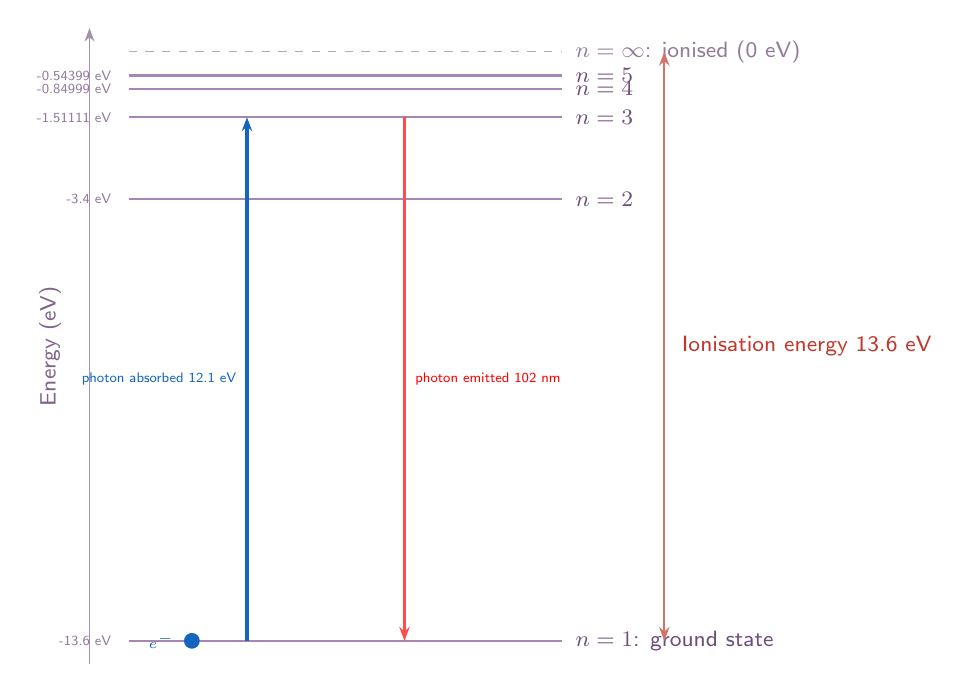
\begin{tikzpicture}[every node/.style={font=\sffamily\small}, scale=1.0]
  % Energy level summary diagram
  \pgfmathsetmacro{\sc}{0.55}

  % Draw levels
  \foreach \n/\lbl in {1/{$n=1$: ground state},
                        2/{$n=2$},
                        3/{$n=3$},
                        4/{$n=4$},
                        5/{$n=5$}} {
    \pgfmathsetmacro{\y}{-13.6/(\n*\n)*\sc}
    \draw[thick, ModuleColor!60] (0,\y) -- (5.5,\y);
    \node[right, font=\sffamily\footnotesize, text=JourneyColor!80]
      at (5.55,\y) {\lbl};
    \pgfmathsetmacro{\En}{-13.6/(\n*\n)}
    \node[left, font=\sffamily\tiny, text=JourneyColor!60]
      at (-0.1,\y) {\En\ eV};
  }

  % n=infinity (ionisation)
  \draw[dashed, thin, JourneyColor!40] (0,0) -- (5.5,0);
  \node[right, font=\sffamily\footnotesize, text=JourneyColor!60]
    at (5.55,0) {$n=\infty$: ionised (0 eV)};

  % Ionisation energy arrow
  \draw[{Stealth[length=5pt]}-{Stealth[length=5pt]}, thick, WarningColor!70]
    (6.8,-7.48) -- (6.8,0);
  \node[right, font=\sffamily\footnotesize, text=WarningColor]
    at (6.9,-3.74) {Ionisation energy 13.6 eV};

  % Excitation arrow (n=1 -> n=3)
  \draw[-{Stealth[length=5pt]}, thick, ElectronBlue, line width=1.2pt]
    (1.5,-7.48) -- (1.5,-0.831)
    node[midway, left, font=\sffamily\tiny, text=ElectronBlue]
    {photon absorbed 12.1 eV};

  % De-excitation arrow (n=3 -> n=1)
  \draw[-{Stealth[length=5pt]}, thick, red!70, line width=1.2pt]
    (3.5,-0.831) -- (3.5,-7.48)
    node[midway, right, font=\sffamily\tiny, text=red]
    {photon emitted 102 nm};

  % Ground state electron
  \fill[ElectronBlue] (0.8,-7.48) circle (0.10cm);
  \node[font=\sffamily\tiny, text=ElectronBlue, left]
    at (0.7,-7.48) {$e^-$};

  % Energy axis
  \draw[-{Stealth}, thin, JourneyColor!50] (-0.5,-7.78) -- (-0.5,0.3);
  \node[rotate=90, font=\sffamily\footnotesize, text=JourneyColor!70]
    at (-1.0,-3.74) {Energy (eV)};
\end{tikzpicture}
\end{center}

% ─── Section: Multi-electron Atoms ───────────────────────────────────────────
\subsection{Extension: Bohr Model for Hydrogen-Like Ions}

The Bohr model works exactly for any ion with a single electron.
For a nucleus with atomic number $Z$, the Coulomb force
is $Z$ times stronger, so all energies scale as $Z^2$:

\[
  E_n^{(Z)} = -\frac{13.6\, Z^2}{n^2}\ \text{eV}
  \qquad
  r_n^{(Z)} = \frac{n^2 a_0}{Z}
\]

\begin{center}
\begin{tabular}{llcc}
\toprule
Ion & $Z$ & Ground state energy & Ionisation energy \\
\midrule
H    & 1 & $-13.6$ eV & 13.6 eV \\
He$^+$ & 2 & $-54.4$ eV & 54.4 eV \\
Li$^{2+}$ & 3 & $-122.4$ eV & 122.4 eV \\
C$^{5+}$ & 6 & $-489.6$ eV & 489.6 eV \\
\bottomrule
\end{tabular}
\end{center}

\vspace{0.5em}

Notice the pattern: the ionisation energy scales as $Z^2$.
This means it takes 4 times more energy to ionise \ce{He+}
than hydrogen, and 9 times more to ionise \ce{Li^{2+}}.

For multi-electron atoms (He, Li, C, \ldots), the model
fails because electrons repel each other.
The exact treatment requires solving the multi-body
Schr\"{o}dinger equation.

\begin{problembox}
\begin{enumerate}[label=\textbf{\arabic*.}]
  \item For singly-ionised helium \ce{He+} ($Z=2$):
        \begin{enumerate}[label=(\alph*)]
          \item Calculate the ground-state orbital radius.
                How does it compare to hydrogen?
          \item Calculate the wavelength of the $n=2 \to n=1$
                transition. In which spectral series does this
                fall (Lyman analogue)?
          \item Calculate the ionisation energy in eV and in
                kJ/mol.
          \item At what temperature would $k_BT$ equal
                the ionisation energy of \ce{He+}?
                Such temperatures occur in stellar coronae.
        \end{enumerate}

  \item The \textbf{Pickering series} consists of lines of
        \ce{He+} with $n_1 = 4$.
        \begin{enumerate}[label=(\alph*)]
          \item Calculate the first three wavelengths
                ($n_2 = 5, 6, 7$) of this series.
          \item Some Pickering lines fall very close to
                Balmer lines of hydrogen.
                Find which Pickering line ($n_2$) is closest
                to H$\alpha$ (656.3 nm) and calculate
                the wavelength difference.
          \item Early astrophysicists mistakenly attributed
                Pickering lines to hydrogen.
                Explain why this confusion arose and
                how it was resolved.
        \end{enumerate}

  \item A muonic hydrogen atom has a muon
        (mass $m_\mu = 207\,m_e$, charge $-e$)
        orbiting a proton instead of an electron.
        \begin{enumerate}[label=(\alph*)]
          \item By what factor does the Bohr radius change?
          \item By what factor does the ground-state energy change?
          \item In what spectral region do muonic hydrogen
                transitions fall?
          \item Why might muonic atoms be useful for measuring
                the proton radius precisely?
        \end{enumerate}
\end{enumerate}
\end{problembox}

% ─── Section: Why Bohr's Model Works ─────────────────────────────────────────
\subsection{Why Bohr's Model Works: de Broglie's Hint}

Bohr imposed angular momentum quantisation ($L = n\hbar$)
without being able to explain it.
Twelve years later, Louis de Broglie (1924) proposed that
all matter has a wavelength:

\[
  \lambda = \frac{h}{p} = \frac{h}{m_e v}
\]

With this \newterm{de Broglie wavelength}, Bohr's quantisation
rule has a beautiful geometric interpretation.

The allowed orbits are those for which an integer number
of electron wavelengths fits exactly around the circumference:

\[
  2\pi r = n\lambda = \frac{nh}{m_e v}
  \quad\Rightarrow\quad
  m_e v r = \frac{nh}{2\pi} = n\hbar
\]

This is exactly Bohr's quantisation rule --- but now it
has a physical meaning: the electron is a \emph{standing wave}
around the nucleus.

\begin{center}
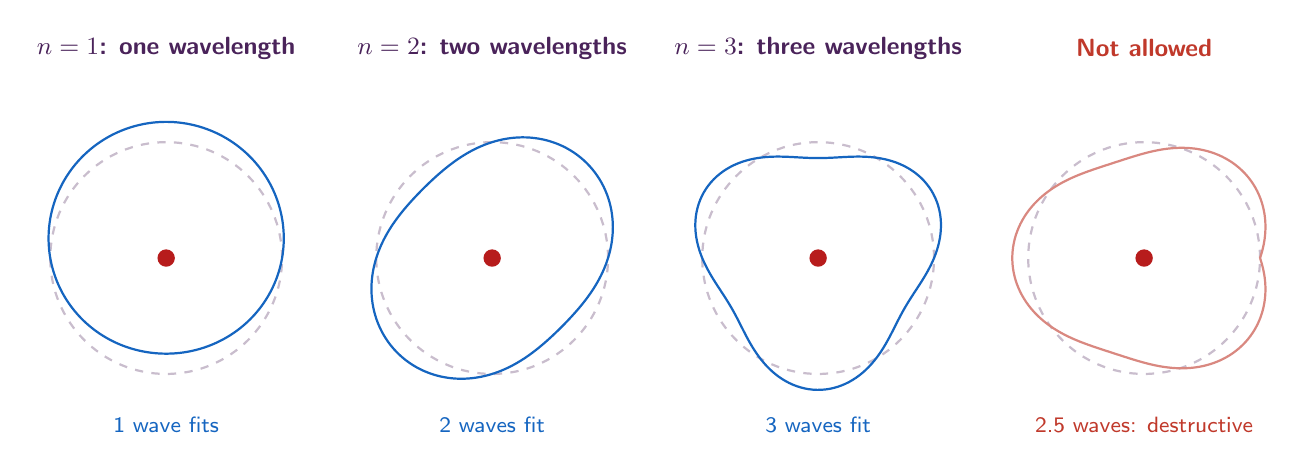
\begin{tikzpicture}[every node/.style={font=\sffamily\small}, scale=0.92]

  % n=1: 1 wavelength around orbit
  \begin{scope}[xshift=-4.5cm]
    \node[font=\sffamily\small\bfseries, color=JourneyColor]
      at (0, 2.9) {$n=1$: one wavelength};
    \draw[thick, JourneyColor!30, dashed] (0,0) circle (1.6cm);
    \fill[NucleusRed] (0,0) circle (0.12cm);
    % Standing wave: r(theta) = r0 + A*sin(1*theta)
    \draw[thick, ElectronBlue, domain=0:360, samples=200]
      plot ({(1.6 + 0.28*sin(\x))*cos(\x)}, {(1.6 + 0.28*sin(\x))*sin(\x)});
    \node[font=\sffamily\footnotesize, text=ElectronBlue] at (0,-2.3) {1 wave fits};
  \end{scope}

  % n=2: 2 wavelengths around orbit
  \begin{scope}[xshift=0cm]
    \node[font=\sffamily\small\bfseries, color=JourneyColor]
      at (0, 2.9) {$n=2$: two wavelengths};
    \draw[thick, JourneyColor!30, dashed] (0,0) circle (1.6cm);
    \fill[NucleusRed] (0,0) circle (0.12cm);
    \draw[thick, ElectronBlue, domain=0:360, samples=200]
      plot ({(1.6 + 0.25*sin(2*\x))*cos(\x)}, {(1.6 + 0.25*sin(2*\x))*sin(\x)});
    \node[font=\sffamily\footnotesize, text=ElectronBlue] at (0,-2.3) {2 waves fit};
  \end{scope}

  % n=3: 3 wavelengths around orbit
  \begin{scope}[xshift=4.5cm]
    \node[font=\sffamily\small\bfseries, color=JourneyColor]
      at (0, 2.9) {$n=3$: three wavelengths};
    \draw[thick, JourneyColor!30, dashed] (0,0) circle (1.6cm);
    \fill[NucleusRed] (0,0) circle (0.12cm);
    \draw[thick, ElectronBlue, domain=0:360, samples=200]
      plot ({(1.6 + 0.22*sin(3*\x))*cos(\x)}, {(1.6 + 0.22*sin(3*\x))*sin(\x)});
    \node[font=\sffamily\footnotesize, text=ElectronBlue] at (0,-2.3) {3 waves fit};
  \end{scope}

  % Non-allowed orbit
  \begin{scope}[xshift=9.0cm]
    \node[font=\sffamily\small\bfseries, color=WarningColor]
      at (0, 2.9) {Not allowed};
    \draw[thick, JourneyColor!30, dashed] (0,0) circle (1.6cm);
    \fill[NucleusRed] (0,0) circle (0.12cm);
    % Partial wave -- destructive interference
    \draw[thick, WarningColor!60, domain=0:360, samples=200]
      plot ({(1.6 + 0.22*sin(2.5*\x))*cos(\x)}, {(1.6 + 0.22*sin(2.5*\x))*sin(\x)});
    \node[font=\sffamily\footnotesize, text=WarningColor]
      at (0,-2.3) {2.5 waves: destructive};
  \end{scope}

\end{tikzpicture}
\end{center}

\vspace{0.5em}

When an integer number of wavelengths fits around the orbit,
the wave reinforces itself --- a stable \newterm{standing wave}.
When a non-integer number would fit, the wave interferes
destructively with itself and cancels --- no stable orbit exists.

This picture --- the electron as a standing wave ---
is the bridge between Bohr's ad-hoc postulate and the
full wave mechanics of Module~2.6.

\begin{historybox}
\textbf{Bohr Meets Rutherford: The Model Is Born}

Niels Bohr arrived in Rutherford's Manchester laboratory
in March 1912, intending to stay four weeks.
He stayed four months.
During this period he absorbed the nuclear model
and began thinking about the stability problem.

He returned to Copenhagen and spent the following year
working out the model.
He later said that the crucial insight came when a friend
showed him the Balmer formula --- which Bohr had never
seen before.
He reportedly said: ``As soon as I saw Balmer's formula,
the whole thing was immediately clear to me.''

He submitted three papers in 1913.
The first paper, which derived the hydrogen spectrum,
caused an immediate sensation.
Einstein said it was ``one of the greatest discoveries.''
Rutherford was reportedly puzzled by Bohr's use of
Planck's constant but could not argue with the numbers.

Bohr received the Nobel Prize in Physics in 1922 ---
the same year that the limitations of his model
became apparent from the spectra of more complex atoms.
\end{historybox}

% ─── Section: Where the Model Breaks ─────────────────────────────────────────
\subsection*{Where the Bohr Model Breaks}

\begin{modelbreaks}
The Bohr model is a brilliant first approximation, but it fails
in five important ways:

\begin{enumerate}[nosep, leftmargin=2em]
  \item \textbf{Multi-electron atoms.} The model cannot be solved
        exactly for helium or any atom with more than one electron,
        because electron-electron repulsion is not included.

  \item \textbf{Fine structure.} The hydrogen spectrum has closely
        spaced \emph{doublets} (e.g.\ the sodium D-lines).
        Bohr's model predicts single lines.
        The splitting requires relativistic corrections and
        \emph{electron spin} (not in Bohr's model).

  \item \textbf{Zeeman effect.} In a magnetic field, each spectral
        line splits into multiple lines.
        Bohr's circular orbits predict only partial agreement.

  \item \textbf{Intensities.} The model predicts which wavelengths
        are emitted but not how \emph{intense} each line is.
        Some transitions are much brighter than others.
        Explaining intensities requires the full quantum theory.

  \item \textbf{Philosophical foundations.} Bohr's model mixes
        classical orbits (electron moving in a circle)
        with quantum postulates (no radiation in allowed orbits).
        This is internally inconsistent --- you cannot have both.
        The correct theory (Schr\"{o}dinger, 1926) abandons
        classical orbits entirely.
\end{enumerate}

All five failures are resolved by wave mechanics, the subject
of Module~2.6.
\end{modelbreaks}

% ─── Section: Deep Problems ───────────────────────────────────────────────────
\subsection*{Deep Problems}

\begin{deepbox}
\begin{enumerate}[label=\textbf{D\arabic*.}]

  \item \textbf{Deriving the Bohr radius from scratch.}

        Starting only from:
        \begin{itemize}[nosep]
          \item $m_e = 9.109\times10^{-31}$ kg
          \item $e = 1.602\times10^{-19}$ C
          \item $\varepsilon_0 = 8.854\times10^{-12}$ C$^2$N$^{-1}$m$^{-2}$
          \item $\hbar = 1.055\times10^{-34}$ Js
        \end{itemize}
        \begin{enumerate}[label=(\alph*)]
          \item Derive $a_0$ from the expression
                $a_0 = 4\pi\varepsilon_0\hbar^2/(m_e e^2)$.
                Calculate its numerical value.
          \item Calculate the ground-state energy $E_1$
                in joules, then convert to eV.
          \item Calculate the Rydberg constant $R_H$ in m$^{-1}$.
          \item From $R_H$, predict the wavelength of H$\alpha$
                (transition $n=3\to n=2$) and compare to the
                measured value 656.3 nm.
        \end{enumerate}

  \item \textbf{The Correspondence Principle in Detail.}

        For the transition $n \to n-1$ at large $n$,
        the frequency of the emitted photon is:
        \[
          \nu_\text{photon} = \frac{R_H c}{1} \cdot
          \frac{(2n-1)}{n^2(n-1)^2}
        \]
        \begin{enumerate}[label=(\alph*)]
          \item For large $n$, show that
                $\nu_\text{photon} \approx 2R_H c / n^3$.
          \item The classical orbital frequency of the electron
                in the $n$-th Bohr orbit is
                $f_\text{classical} = v_n/(2\pi r_n)$.
                Express this in terms of $n$ and fundamental constants.
          \item Show that $\nu_\text{photon} = f_\text{classical}$
                for large $n$.
          \item What is the physical significance of this agreement?
                Why does the quantum formula reduce to the
                classical result for large quantum numbers?
        \end{enumerate}

  \item \textbf{Rydberg Atoms: The Giant Atoms.}

        A Rydberg atom is one in which an electron is promoted
        to a very high principal quantum number, $n \gg 1$.

        \begin{enumerate}[label=(\alph*)]
          \item Calculate the orbital radius of hydrogen
                with $n = 100$. Compare to the wavelength
                of visible light ($\sim 500$ nm).
          \item Calculate the energy spacing between
                levels $n=100$ and $n=101$.
          \item As $n$ increases, the energy spacings become
                very small.
                What does this mean physically for the
                correspondence between classical and quantum
                behaviour?
          \item Rydberg atoms are used in quantum computing
                experiments because they have very large
                electric dipole moments (they interact
                strongly with electric fields).
                Why does a large orbital radius lead to a
                large dipole moment when the atom is placed
                in an electric field?
          \item The lifetime of a Rydberg state scales as $n^3$.
                Estimate the lifetime of $n=100$ hydrogen
                given that $n=2$ has lifetime $\sim 10^{-9}$ s.
        \end{enumerate}

\end{enumerate}
\end{deepbox}

% ─── Reflection ───────────────────────────────────────────────────────────────
\subsection*{Reflection}

\begin{reflectionbox}
\begin{enumerate}[label=\textbf{R\arabic*.}]
  \item Bohr's postulate 1 says electrons do not radiate
        in stationary states.
        This directly contradicts classical electrodynamics.
        \textbf{Was Bohr entitled to make this postulate?}
        Under what circumstances is it legitimate to simply
        assert that an established theory does not apply?
        What would count as justification?

  \item The Bohr model works perfectly for hydrogen and
        completely fails for helium (two electrons).
        \textbf{What does this tell us about the limits of
        models that treat particles as independent?}
        When is the approximation of ignoring interactions
        between particles valid, and when does it break down?

  \item Bohr said he saw the Balmer formula and ``immediately
        the whole thing was clear.''
        \textbf{What does ``clarity'' mean in this context?}
        Had he seen a physical picture, or had he seen a
        mathematical structure?
        Is mathematical insight the same as physical understanding?

  \item The de Broglie picture (standing waves around the orbit)
        explains Bohr's quantisation rule beautifully ---
        but it still describes electrons as having definite
        positions in classical orbits.
        \textbf{What is wrong with this picture,
        and what would a more honest description look like?}
        (Think about what ``standing wave'' actually means
        for a physical object --- Module~2.6 will revisit this.)
\end{enumerate}
\end{reflectionbox}

\vspace{1.5em}
\begin{center}
\begin{tcolorbox}[enhanced, colback=DiscoveryColor!8, colframe=DiscoveryColor,
  width=0.88\textwidth, arc=3pt]
\centering\sffamily\small
\textbf{What we invented in this module.}\\[4pt]
We invented the quantised orbit.
By imposing two conditions --- classical force balance and
quantised angular momentum --- Bohr derived the hydrogen energy
levels, the Rydberg constant, and the Bohr radius from
fundamental constants alone, with no free parameters.
The five-figure agreement with experiment is compelling evidence
that something deep is being captured.
But the model is internally inconsistent: it applies classical
mechanics to orbiting electrons and then tells those electrons
to ignore classical electrodynamics.
The resolution is to abandon the concept of an orbit entirely.
An electron in an atom does not travel in a circle.
It occupies a \emph{probability cloud} described by a wave function.
That is the subject of the next two modules.
\end{tcolorbox}
\end{center}

\vspace{2em}
\noindent\textcolor{JourneyColor!40}{\rule{\textwidth}{0.6pt}}
\begin{center}
\textit{\sffamily\small
Module 2.5 complete. Continue to Module 2.6:\\
\textbf{Wave-Particle Duality and the Quantum Atom}.}
\end{center}

\end{document}